\begin{figure}[h]
	\centerline{$
	\begin{array}{cccc}
	 \emptyset & \{1\}  & \{2\} & \{1,2\}  \\   \\
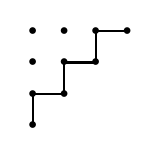
\begin{tikzpicture}[scale=.4, baseline=.5cm]
	\foreach \y in {0,1,2,3}
		\node (0,\y) at (0,\y) [inner sep=0pt] {$\scriptscriptstyle \bullet$};
	\foreach \y in {1,2,3}
		\node (1,\y) at (1,\y) [inner sep=0pt] {$\scriptscriptstyle \bullet$};
	\foreach \y in {2,3}
		\node (2,\y) at (2,\y) [inner sep=0pt] {$\scriptscriptstyle \bullet$};
	\node (3,3) at (3,3) [inner sep=0pt] {$\scriptscriptstyle \bullet$};
	\draw [thick] (0,0)--(0,1); 
	\draw [thick] (0,1)--(1,1); 
	\draw [thick] (1,1)--(1,2); 
	\draw [thick] (1,2)--(2,2); 
	\draw [thick] (2,2)--(2,3); 
	\draw [thick] (2,3)--(3,3); 
\end{tikzpicture} 
 &
 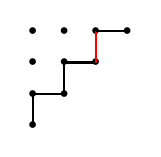
\begin{tikzpicture}[scale=.4, baseline=.5cm]
	\foreach \y in {0,1,2,3}
		\node (0,\y) at (0,\y) [inner sep=0pt] {$\scriptscriptstyle \bullet$};
	\foreach \y in {1,2,3}
		\node (1,\y) at (1,\y) [inner sep=0pt] {$\scriptscriptstyle \bullet$};
	\foreach \y in {2,3}
		\node (2,\y) at (2,\y) [inner sep=0pt] {$\scriptscriptstyle \bullet$};
	\node (3,3) at (3,3) [inner sep=0pt] {$\scriptscriptstyle \bullet$};
	\draw [thick] (0,0)--(0,1); 
	\draw [thick] (0,1)--(1,1); 
	\draw [thick] (1,1)--(1,2); 
	\draw [thick] (1,2)--(2,2); 
	\draw [thick,color=red] (2,2)--(2,3); 
	\draw [thick] (2,3)--(3,3); 
\end{tikzpicture} 
&
 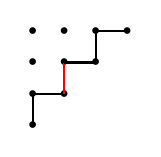
\begin{tikzpicture}[scale=.4, baseline=.5cm]
	\foreach \y in {0,1,2,3}
		\node (0,\y) at (0,\y) [inner sep=0pt] {$\scriptscriptstyle \bullet$};
	\foreach \y in {1,2,3}
		\node (1,\y) at (1,\y) [inner sep=0pt] {$\scriptscriptstyle \bullet$};
	\foreach \y in {2,3}
		\node (2,\y) at (2,\y) [inner sep=0pt] {$\scriptscriptstyle \bullet$};
	\node (3,3) at (3,3) [inner sep=0pt] {$\scriptscriptstyle \bullet$};
	\draw [thick] (0,0)--(0,1); 
	\draw [thick] (0,1)--(1,1); 
	\draw [thick,color=red] (1,1)--(1,2); 
	\draw [thick] (1,2)--(2,2); 
	\draw [thick] (2,2)--(2,3); 
	\draw [thick] (2,3)--(3,3); 
\end{tikzpicture} 
&
 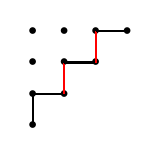
\begin{tikzpicture}[scale=.4, baseline=.5cm]
	\foreach \y in {0,1,2,3}
		\node (0,\y) at (0,\y) [inner sep=0pt] {$\scriptscriptstyle \bullet$};
	\foreach \y in {1,2,3}
		\node (1,\y) at (1,\y) [inner sep=0pt] {$\scriptscriptstyle \bullet$};
	\foreach \y in {2,3}
		\node (2,\y) at (2,\y) [inner sep=0pt] {$\scriptscriptstyle \bullet$};
	\node (3,3) at (3,3) [inner sep=0pt] {$\scriptscriptstyle \bullet$};
	\draw [thick] (0,0)--(0,1); 
	\draw [thick] (0,1)--(1,1); 
	\draw [thick,color=red] (1,1)--(1,2); 
	\draw [thick] (1,2)--(2,2); 
	\draw [thick,color=red] (2,2)--(2,3); 
	\draw [thick] (2,3)--(3,3); 
\end{tikzpicture} 
 \\
		\\
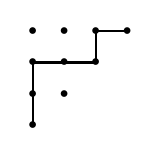
\begin{tikzpicture}[scale=.4, baseline=.5cm]
	\foreach \y in {0,1,2,3}
		\node (0,\y) at (0,\y) [inner sep=0pt] {$\scriptscriptstyle \bullet$};
	\foreach \y in {1,2,3}
		\node (1,\y) at (1,\y) [inner sep=0pt] {$\scriptscriptstyle \bullet$};
	\foreach \y in {2,3}
		\node (2,\y) at (2,\y) [inner sep=0pt] {$\scriptscriptstyle \bullet$};
	\node (3,3) at (3,3) [inner sep=0pt] {$\scriptscriptstyle \bullet$};
	\draw [thick] (0,0)--(0,1); 
	\draw [thick] (0,1)--(0,2); 
	\draw [thick] (0,2)--(1,2); 
	\draw [thick] (1,2)--(2,2); 
	\draw [thick] (2,2)--(2,3); 
	\draw [thick] (2,3)--(3,3); 
\end{tikzpicture} 
&
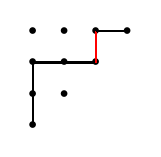
\begin{tikzpicture}[scale=.4, baseline=.5cm]
	\foreach \y in {0,1,2,3}
		\node (0,\y) at (0,\y) [inner sep=0pt] {$\scriptscriptstyle \bullet$};
	\foreach \y in {1,2,3}
		\node (1,\y) at (1,\y) [inner sep=0pt] {$\scriptscriptstyle \bullet$};
	\foreach \y in {2,3}
		\node (2,\y) at (2,\y) [inner sep=0pt] {$\scriptscriptstyle \bullet$};
	\node (3,3) at (3,3) [inner sep=0pt] {$\scriptscriptstyle \bullet$};
	\draw [thick] (0,0)--(0,1); 
	\draw [thick] (0,1)--(0,2); 
	\draw [thick] (0,2)--(1,2); 
	\draw [thick] (1,2)--(2,2); 
	\draw [thick,color=red] (2,2)--(2,3); 
	\draw [thick] (2,3)--(3,3); 
\end{tikzpicture} 
&
                    	& \\
		\\
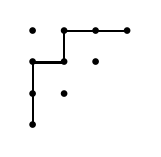
\begin{tikzpicture}[scale=.4, baseline=.5cm]
	\foreach \y in {0,1,2,3}
		\node (0,\y) at (0,\y) [inner sep=0pt] {$\scriptscriptstyle \bullet$};
	\foreach \y in {1,2,3}
		\node (1,\y) at (1,\y) [inner sep=0pt] {$\scriptscriptstyle \bullet$};
	\foreach \y in {2,3}
		\node (2,\y) at (2,\y) [inner sep=0pt] {$\scriptscriptstyle \bullet$};
	\node (3,3) at (3,3) [inner sep=0pt] {$\scriptscriptstyle \bullet$};
	\draw [thick] (0,0)--(0,1); 
	\draw [thick] (0,1)--(0,2); 
	\draw [thick] (0,2)--(1,2); 
	\draw [thick] (1,2)--(1,3); 
	\draw [thick] (1,3)--(2,3); 
	\draw [thick] (2,3)--(3,3); 
\end{tikzpicture} 
 & &
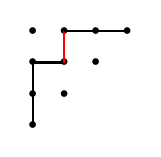
\begin{tikzpicture}[scale=.4, baseline=.5cm]
	\foreach \y in {0,1,2,3}
		\node (0,\y) at (0,\y) [inner sep=0pt] {$\scriptscriptstyle \bullet$};
	\foreach \y in {1,2,3}
		\node (1,\y) at (1,\y) [inner sep=0pt] {$\scriptscriptstyle \bullet$};
	\foreach \y in {2,3}
		\node (2,\y) at (2,\y) [inner sep=0pt] {$\scriptscriptstyle \bullet$};
	\node (3,3) at (3,3) [inner sep=0pt] {$\scriptscriptstyle \bullet$};
	\draw [thick] (0,0)--(0,1); 
	\draw [thick] (0,1)--(0,2); 
	\draw [thick] (0,2)--(1,2); 
	\draw [thick,color=red] (1,2)--(1,3); 
	\draw [thick] (1,3)--(2,3); 
	\draw [thick] (2,3)--(3,3); 
\end{tikzpicture} 
& \\
		\\
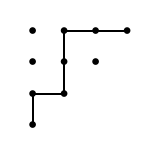
\begin{tikzpicture}[scale=.4, baseline=.5cm]
	\foreach \y in {0,1,2,3}
		\node (0,\y) at (0,\y) [inner sep=0pt] {$\scriptscriptstyle \bullet$};
	\foreach \y in {1,2,3}
		\node (1,\y) at (1,\y) [inner sep=0pt] {$\scriptscriptstyle \bullet$};
	\foreach \y in {2,3}
		\node (2,\y) at (2,\y) [inner sep=0pt] {$\scriptscriptstyle \bullet$};
	\node (3,3) at (3,3) [inner sep=0pt] {$\scriptscriptstyle \bullet$};
	\draw [thick] (0,0)--(0,1); 
	\draw [thick] (0,1)--(1,1); 
	\draw [thick] (1,1)--(1,2); 
	\draw [thick] (1,2)--(1,3); 
	\draw [thick] (1,3)--(2,3); 
	\draw [thick] (2,3)--(3,3); 
\end{tikzpicture} 
&
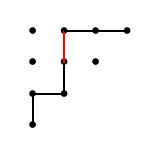
\begin{tikzpicture}[scale=.4, baseline=.5cm]
	\foreach \y in {0,1,2,3}
		\node (0,\y) at (0,\y) [inner sep=0pt] {$\scriptscriptstyle \bullet$};
	\foreach \y in {1,2,3}
		\node (1,\y) at (1,\y) [inner sep=0pt] {$\scriptscriptstyle \bullet$};
	\foreach \y in {2,3}
		\node (2,\y) at (2,\y) [inner sep=0pt] {$\scriptscriptstyle \bullet$};
	\node (3,3) at (3,3) [inner sep=0pt] {$\scriptscriptstyle \bullet$};
	\draw [thick] (0,0)--(0,1); 
	\draw [thick] (0,1)--(1,1); 
	\draw [thick] (1,1)--(1,2); 
	\draw [thick,color=red] (1,2)--(1,3); 
	\draw [thick] (1,3)--(2,3); 
	\draw [thick] (2,3)--(3,3); 
\end{tikzpicture} 
&
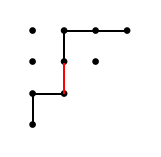
\begin{tikzpicture}[scale=.4, baseline=.5cm]
	\foreach \y in {0,1,2,3}
		\node (0,\y) at (0,\y) [inner sep=0pt] {$\scriptscriptstyle \bullet$};
	\foreach \y in {1,2,3}
		\node (1,\y) at (1,\y) [inner sep=0pt] {$\scriptscriptstyle \bullet$};
	\foreach \y in {2,3}
		\node (2,\y) at (2,\y) [inner sep=0pt] {$\scriptscriptstyle \bullet$};
	\node (3,3) at (3,3) [inner sep=0pt] {$\scriptscriptstyle \bullet$};
	\draw [thick] (0,0)--(0,1); 
	\draw [thick] (0,1)--(1,1); 
	\draw [thick,color=red] (1,1)--(1,2); 
	\draw [thick] (1,2)--(1,3); 
	\draw [thick] (1,3)--(2,3); 
	\draw [thick] (2,3)--(3,3); 
\end{tikzpicture} 
&  \\
		\\
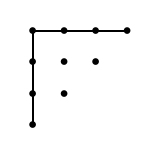
\begin{tikzpicture}[scale=.4, baseline=.5cm]
	\foreach \y in {0,1,2,3}
		\node (0,\y) at (0,\y) [inner sep=0pt] {$\scriptscriptstyle \bullet$};
	\foreach \y in {1,2,3}
		\node (1,\y) at (1,\y) [inner sep=0pt] {$\scriptscriptstyle \bullet$};
	\foreach \y in {2,3}
		\node (2,\y) at (2,\y) [inner sep=0pt] {$\scriptscriptstyle \bullet$};
	\node (3,3) at (3,3) [inner sep=0pt] {$\scriptscriptstyle \bullet$};
	\draw [thick] (0,0)--(0,1); 
	\draw [thick] (0,1)--(0,2); 
	\draw [thick] (0,2)--(0,3); 
	\draw [thick] (0,3)--(1,3); 
	\draw [thick] (1,3)--(2,3); 
	\draw [thick] (2,3)--(3,3); 
\end{tikzpicture} 
& & & \\
        \end{array}
 	$}
	\caption{Decomposition of $\Xi_3$}
	\label{fig:decompositionPath3}
\end{figure}